%%%%%%%%%%%%%%%%%%%%%%%%%%%%%%%%%%%%%%%%%
% University/School Laboratory Report
% LaTeX Template
% Version 3.1 (25/3/14)
%
% This template has been downloaded from:
% http://www.LaTeXTemplates.com
%
% Original author:
% Linux and Unix Users Group at Virginia Tech Wiki 
% (https://vtluug.org/wiki/Example_LaTeX_chem_lab_report)
%
% License:
% CC BY-NC-SA 3.0 (http://creativecommons.org/licenses/by-nc-sa/3.0/)
%
%%%%%%%%%%%%%%%%%%%%%%%%%%%%%%%%%%%%%%%%%

%----------------------------------------------------------------------------------------
%	PACKAGES AND DOCUMENT CONFIGURATIONS
%----------------------------------------------------------------------------------------

\documentclass{article}

\usepackage[version=3]{mhchem} % Package for chemical equation typesetting
\usepackage{siunitx} % Provides the \SI{}{} and \si{} command for typesetting SI units
\usepackage{graphicx} % Required for the inclusion of images
\usepackage{natbib} % Required to change bibliography style to APA
\usepackage{amsmath} % Required for some math elements 

\setlength\parindent{0pt} % Removes all indentation from paragraphs

\renewcommand{\labelenumi}{\alph{enumi}.} % Make numbering in the enumerate environment by letter rather than number (e.g. section 6)

%\usepackage{times} % Uncomment to use the Times New Roman font

%----------------------------------------------------------------------------------------
%	DOCUMENT INFORMATION
%----------------------------------------------------------------------------------------

\title{CPA Lab-Report \\ Lab 2 Prime Numbers} % Title

\author{Simon \textsc{Birrer}, Dominic \textsc{Sch\"urmann}} % Author name

\date{\today} % Date for the report

\begin{document}

\maketitle % Insert the title, author and date

\begin{center}
\begin{tabular}{l r}
Date Performed: & October 27, 2015 \\ % Date the experiment was performed
Partners: & Simon Birrer \\ % Partner names
& Dominic Sch\"umann \\
Instructor: & Professor Smith % Instructor/supervisor
\end{tabular}
\end{center}

\bigskip

\tableofcontents

\pagebreak

\section{Biggest prime storable in 8 bytes}

\subsection{Compiling without OpenMP}
\subsection{Time measurement of parallelized version}

\begin{figure}[ht]
	\centering
  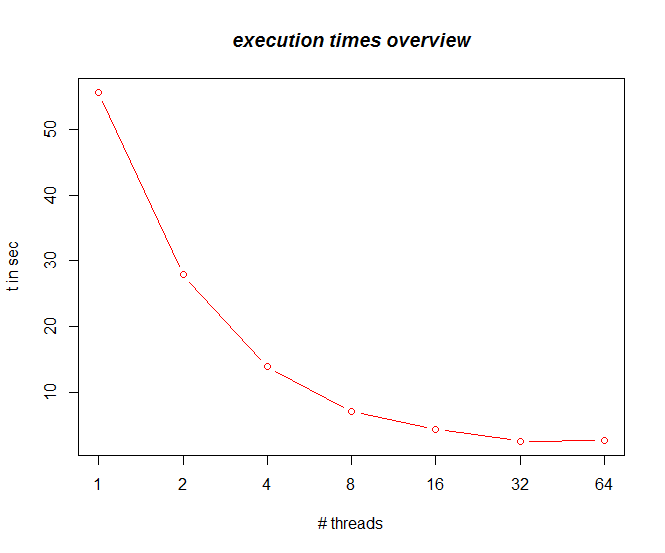
\includegraphics[width=0.9\textwidth]{statistics/Ex12ResultGraph.png}
	\caption{execution times for exercise 1.2}
\end{figure}

\begin{figure}[ht]
	\centering
  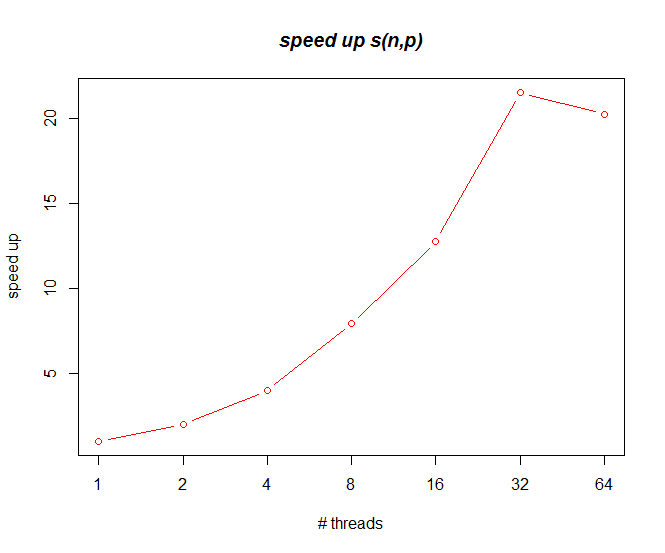
\includegraphics[width=0.9\textwidth]{statistics/Ex12SpeedUpGraph.png}
	\caption{speed up for exercise 1.2}
\end{figure}

\section{Count primes in a range}

\subsection{Exercise 1 with reduction clause}

\subsubsection{scheduling distribution}

\begin{enumerate}
\item static 0, without chunk
\item static 1, with chunk
\item dynamic
\end{enumerate}

\subsection{Exercise 2 printing workload}

%----------------------------------------------------------------------------------------
%	BIBLIOGRAPHY
%----------------------------------------------------------------------------------------

\bibliographystyle{apalike}

\bibliography{sample}

%----------------------------------------------------------------------------------------


\end{document}